\section{Software Framework and Tools}
\label{sec:framework}

Nuclear and particle physics data processing applications must guarantee a long lifetime.  Larger than the multi-year
duration of the corresponding experiment. The ability to upgrade and adapt technologies is therefore essential, so
these applications should be organized in a way that easily permits upgrades of aged software components and
inclusion of new ones, without need for major redesign or structural changes.  Support for software evolution and
diversification (e.g. compatibility with heterogeneous hardware structures, such as FPGAs and GPGPUs) is important
to accommodate more efficient and robust data processing applications in the future.

Following these principles, CLAS12 reconstruction and analysis relies on a data-stream processing framework called
CLARA~\cite{clara-2011,clara-service,framework,clara-2016}, which provides a service-oriented architecture in which
to build the relevant software applications.  Such applications are composed of interlocking building blocks called
micro-services, which are linked together by data-stream pipes.  The technology (e.g. a high-level programming
language or hardware deployment details), as well as the algorithmic solutions used to process data are encapsulated. 
The scope of a specific software application implemented in CLARA is determined
by the micro-services that are included and by the order of their execution.

A micro-service receives input data, processes it, and produces output data, where the I/O is organized into  tabular structures called a ``banks''
whose structure is configured by the specific service developer.  A micro-service reacts to an input data stream,
processes it, and passes processed data to the next micro-service in the data-flow path.  As a result, the CLAS12
data processing application is versatile and flexible, since the application building blocks can be improved individually
and replaced with no need for structural changes in the framework. The CLAS12 micro-services are extensions of an
abstract reconstruction engine, which includes common components such as initialization and event processing
methods. This approach reduces and simplifies the development of an individual micro-service and enforces a common
structure. 

The CLARA data-stream pipe is a data bus based on the xMsg messaging system that supports various protocols
such as MPI, pub-sub, p2p, inproc, and shared memory. The CLARA orchestrator, i.e. the process level workflow
management system, controls the overall process execution. 

The framework enables execution of software applications in multi-threaded mode. This is implemented via event-level
parallelization for the CLAS12 reconstruction. 
The framework is specifically designed to do thread-based
parallelization on multicore machines, thereby allowing 
the simultaneous reconstruction of multiple events having as many active threads as the cores
on the system.  
Figure~\ref{fig:scaling} shows the results of a scaling test on an
Intel Xeon node (E5-2697A v4 @ 2.6~GHz). Comparison with Amdhal's law indicates 99.5\% parallel efficiency over
the 32 physical cores of the machine.

The CLARA framework provides service interface implementations in Java, C++ and Python languages. 
At present, all the CLAS12 reconstruction services deployed using the CLARA framework are written in Java.

\begin{figure}
\centering
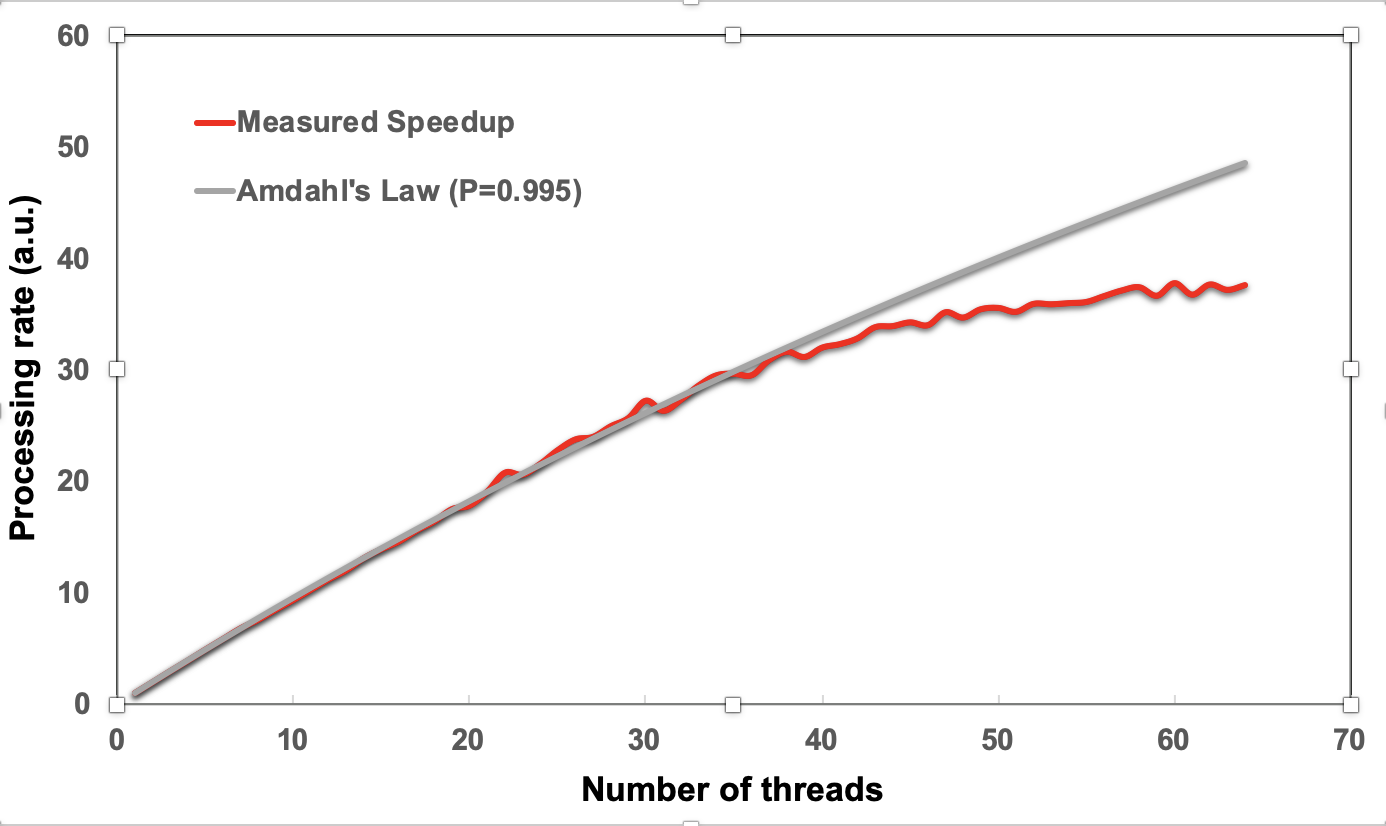
\includegraphics[width=0.48\textwidth]{pics/scaling.png}
\caption{Scaling of the CLAS12 full event reconstruction application as implemented in the CLARA framework. Tests
  were conducted on a Intel Xeon node (E5-2697A v4 @ 2.6~GHz). Comparison with Amdhal's law indicates 99.5\%
  parallel efficiency over the 32 physical cores of the machine.}
\label{fig:scaling}
\end{figure}

\subsection{Common Tools}
\label{common-tools}

The offline software of the CLAS12 project aims to provide tools that allow design, simulation, and data analysis
to proceed in an efficient, repeatable, and understandable way. Most  software engineering details are hidden from
users, allowing them to concentrate on the algorithms and physics. To facilitate code development for the detector
subsystems of CLAS12, the software was designed to provide libraries that are commonly used by all of the
reconstruction packages.  These libraries, referred to as ``common tools'',  contribute to software maintainability 
by avoiding code replication, which facilitates code maintainability.

The common tools consist of various packages, each having a specific purpose and functionality. Below we discuss
the main packages used in the reconstruction software.

\subsubsection{Geometry}

Due to the complexity of the geometry of the CLAS12 detector subsystems, an interface was developed to provide
classes and software tools that are used to describe the geometry of all subsystems in an unified way.  A library of
primitives provides geometrical objects needed to represent all detector subsystems (these include lines, planes,
and various shapes such as cubes, trapezoids, etc.) and provide the necessary transformations to accommodate
misalignments and distortions.  Furthermore, geometry tools provide methods to track particles through volumes for
evaluation of track trajectories, such as line-to-surface intersections, ray tracing through objects, and evaluation of
the distance of closest approach to a line or surface.

The CLAS12 geometry library is initialized from a database containing key geometry parameters and their
variations for every detector.  This maximizes flexibility, supports time-dependent experiment geometry
conditions, and ensures consistency between the simulation, reconstruction, and event visualization packages.

To facilitate development of new detector geometries, visualization capabilities are included in the geometry library.
Figure~\ref{fig:detectorview} shows a view of part of the CLAS12 spectrometer using this functionality.

\subsubsection{Databases}

The Calibration Constant Database (CCDB) software package was developed at Jefferson Lab for the GlueX
experiment in Hall~D~\cite{gluex}.  CCDB provides the functionality for storing and accessing structured tables in
MySQL-based and SQLite portable databases. The CLAS12 reconstruction packages use the CCDB application
programming interface to create and access tables that contain detector geometry and calibration constants, as
well as maps used for decoding raw data. At the decoding stage, the signal is converted from the hardware notation
(crate, slot, channel) into the CLAS12 notation (sector, layer, component). 

The constants in CCDB tables are linked  to specific runs (using time stamps), so that different
variations of constants are stored depending on run conditions. CLAS12 software tools employ an Application Programming
Interface (API) that parses database tables and creates structured maps of constants stored in  memory by
detector sector, layer, and component. This allows fast retrieval of the constants.

The CLAS12 database access tools have been developed to avoid bottlenecks that might result from multiple
multi-threaded services accessing the database to retrieve constants.  An interface has been designed to fetch
the constants on demand and cache them for further requests. In this approach each service will request the
constants it requires on one thread and each subsequent request by a new thread accesses
the cached values.

\subsubsection{Plotting and Analysis Tools}

For ease of integration with the reconstruction software tools and packages, the plotting tools used for data
calibration, monitoring, and analysis were developed in the Java programming language.

The plotting software, called {\it groot}, developed at Jefferson Lab for CLAS12 is tailored to have a programming
interface similar to the CERN data analysis package, ROOT, and provides the necessary functionalities for
histogram and graph creation, filling, and manipulation, as well as for fitting using the Java-based MINUIT library
available from the JHEP repositories. This has been the base for the development of the detector monitoring and
calibration suites (see Section~\ref{sec:calibration}).

These same tools can also be used for physics analysis.
An additional analysis package containing classes for
four-vector manipulations allows computation of event kinematics such as $Q^2$ and $W$ and Lorentz
boosts, etc. 

\begin{figure}
\centering
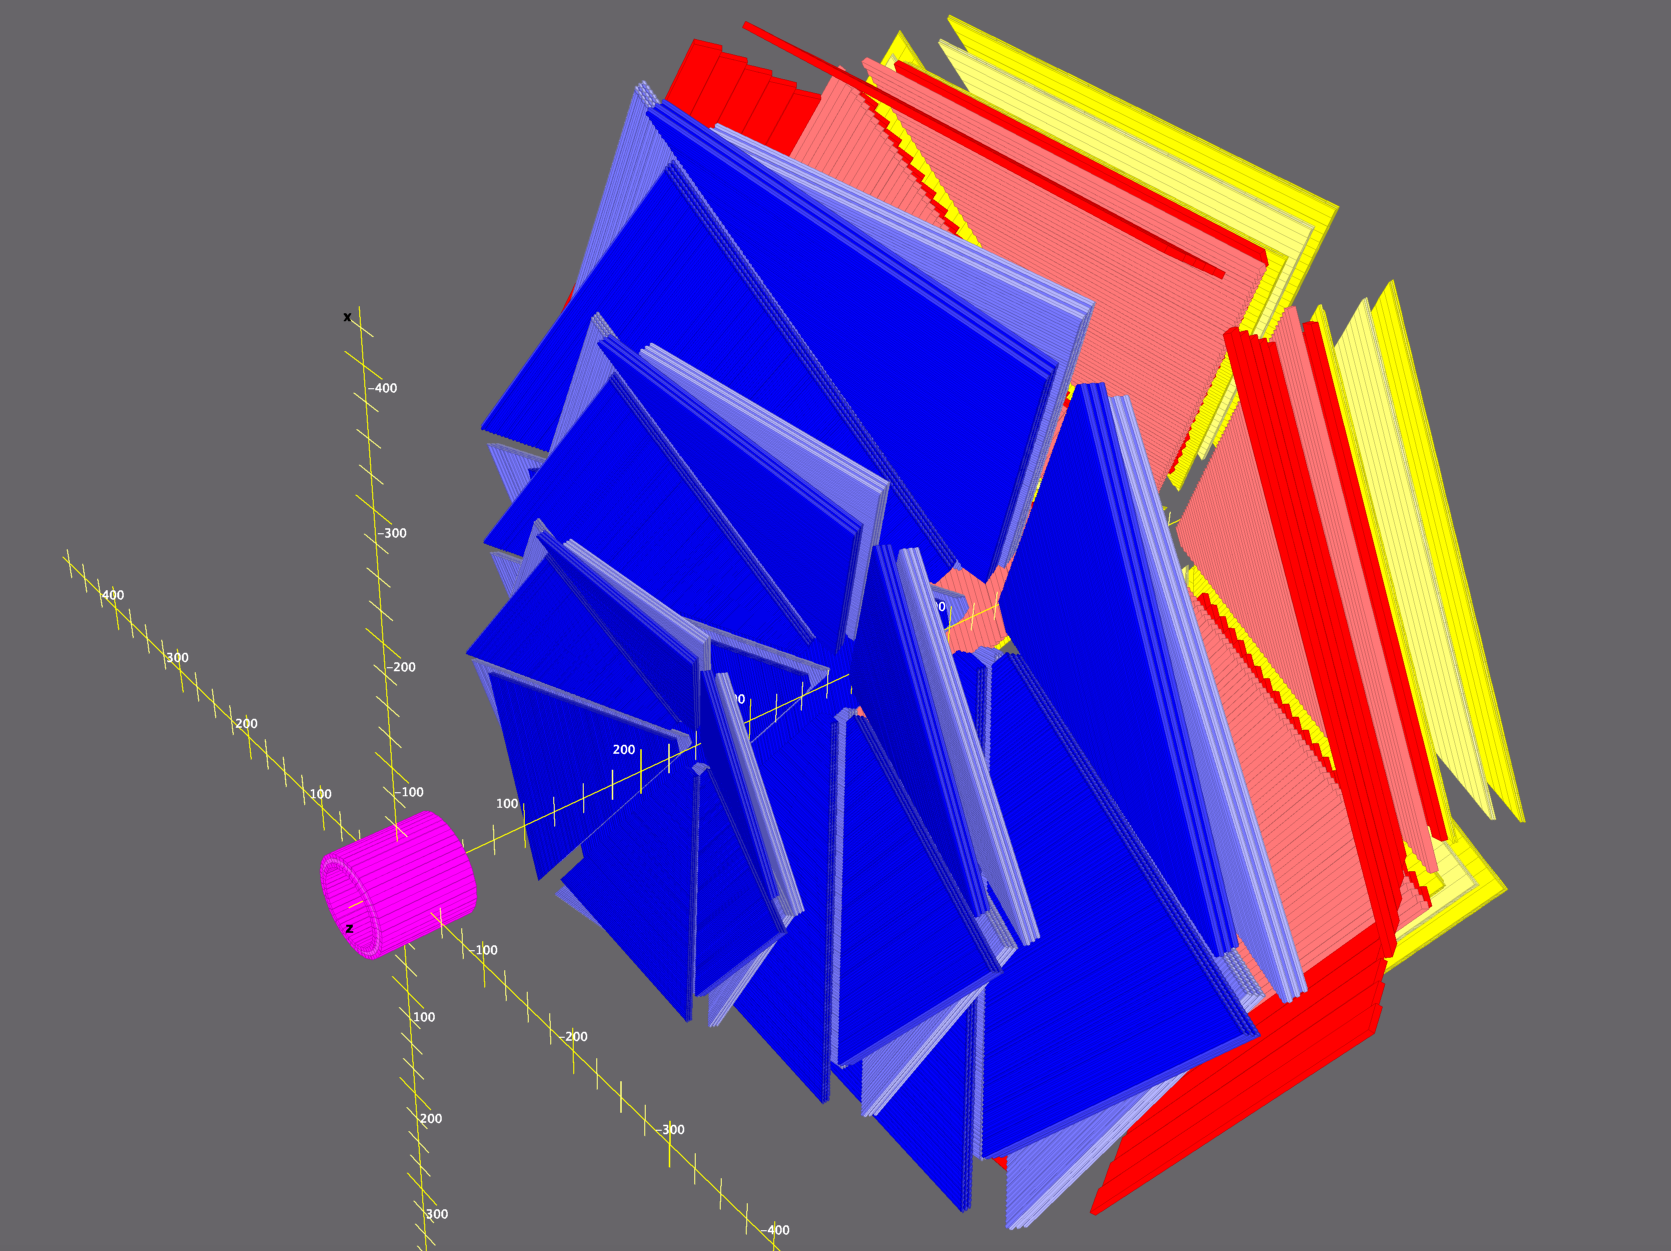
\includegraphics[width=1.0\columnwidth]{pics/detectorview.png}
\caption{Visualization of part of the CLAS12 spectrometer via the geometry package. From left to right, the Central
  Neutron Detector (CND) in magenta, the Drift Chambers (DC) in blue, the Forward Time of Flight (FTOF) in red,
  and the Electromagnetic Calorimeter (ECAL) in yellow are shown.}
\label{fig:detectorview}
\end{figure}

\subsubsection{Magnetic Field Package}

The magnetic field package, {\it magfield}, used by the CLAS12 reconstruction creates binary field maps from
engineering models of the CLAS12 torus and solenoid~\cite{magnets-nim}. It employs a common self-described
binary format, with a header containing meta-data describing the pedigree of the field, its grid coordinate system,
and the coordinate system of the field components. For example, the CLAS12 torus has a cylindrical grid but
Cartesian field components. The same {\it magfield} package provides the trilinear interpolation of the field (a
method of multivariate interpolation on a 3-dimensional regular grid). Given that the field is often requested at a
sequence of points all contained within a single grid cell, {\it magfield} uses time-saving software “probes” to cache
nearest neighbors.

\subsubsection{Swimmer Package}

The {\it swimmer} package, in conjunction with the {\it magfield} package, is used in the CLAS12 reconstruction
to propagate charged particles through the CLAS12 solenoid and torus fields. It uses a fourth-order (with
fifth-order corrections) adaptive step-size Runge-Kutta integrator with single-step advancement that is achieved through
a configurable Butcher tableau advancer. There are a number of convenience methods for swimming to a plane, to
the closest point on a line, and to a specified value of a given $(x,y,z)$ coordinate. 
For forward swimming in CLAS12 performance is improved by reducing
the dimensionality of the track state vector which
contains the main track parameters (Section~\ref{sec-trackfitting}), by
changing the independent variable from the path length 
to the coordinate along the beamline, which defines the
nominal CLAS12 $z$-axis.
